\documentclass[letterpaper,11pt]{article}

\usepackage{amsthm,amsmath,amssymb}
\usepackage[margin=2.0cm]{geometry}
\usepackage{graphicx,float}
\usepackage{tikz}

\newtheorem{proposition}{Proposition}

\newcommand{\R}{\mathbb{R}}

\author{Jacob Thomas Errington (260636023)}
\title{Assignment \#2 \\ Algorithm Design -- COMP 360}
\date{13 October 2015}

\begin{document}

\maketitle

\begin{enumerate}

    \item Our solution to solving the direction assignment problem using
        maximum flow builds a flow network from the given graph $G = (V, E)$ in
        the following way.

        For each edge $e \in E$ that is undirected, we create a vertex $v_e$
        in the flow network, and create an edge to it from the source with
        capacity $1$. Let $V_1$ be the set of these vertices. For each
        $p_{uv} \in V_1$, we create two vertices -- one is called $q_{uv}$ and
        the other is called $q_{vu}$ -- and we create an edge from $p_{uv}$ to
        each of these with capacity $1$. Let $V_2$ be the set of these
        vertices. Then, for each $v \in V$, i.e. the vertices of the original
        graph, create a vertex $v$ in the flow network and let $V_3$ be the set
        of these new vertices. For each $v \in V_3$, create an edge with
        capacity $1$ from each $q_{uv}$. Finally, for each $v \in V_3$, create
        an edge to the sink with capacity equal to the number of (additional)
        incoming edges required to achieve a balance of incoming and outgoing
        edges on that vertex. If the vertex in question has odd degree, or if
        it has enough edges with predetermined directions such that no balance
        can be achieved, then we immediate abort since no solution would be
        found. If the edges leading into the sink are saturated, then a
        solution has been found, and examining the edges from $V_2$ to $V_3$
        indicates which edges need to be set in which direction.

        The intuition for this solution is the following. The vertices in sets
        $V_1$ and $V_2$ are designed to make maximizing the flow in the network
        choose the direction for each edge in the original graph. Indeed,
        elements of $V_2$ represent the possible choices of direction for their
        corresponding element in $V_1$. The vertices in $V_3$ collect the
        choices to add incoming flow and effectively sum them. That sum in turn
        is the amount of flow that they would output.

        Below is an an simple example graph and its corresponding flow network
        constructed using this procedure.

        \begin{figure}[H]
            \centering

            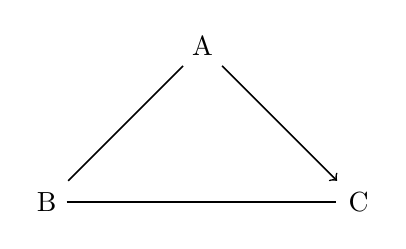
\begin{tikzpicture}[
                    ->,
                    shorten >=1pt,
                    auto,
                    node distance=2.8cm,
                    semithick
                ]
                \node (A) {A} ;
                \node (B) [below left of=A] {B} ;
                \node (C) [below right of=A] {C} ;

                \path
                (A) edge node {} (C)
                ;

                \begin{scope}[-]
                    \path
                    (A) edge node {} (B)
                    (B) edge node {} (C)
                    ;
                \end{scope}
            \end{tikzpicture}

            \label{fig:graph}

            \caption{
                A simple graph with some edges undirected. The direction of
                these edges will be determined by the solution to a maximum
                flow problem on the flow network in figure
                \ref{fig:flownetwork}.
            }
        \end{figure}

        \begin{figure}[H]
            \centering

            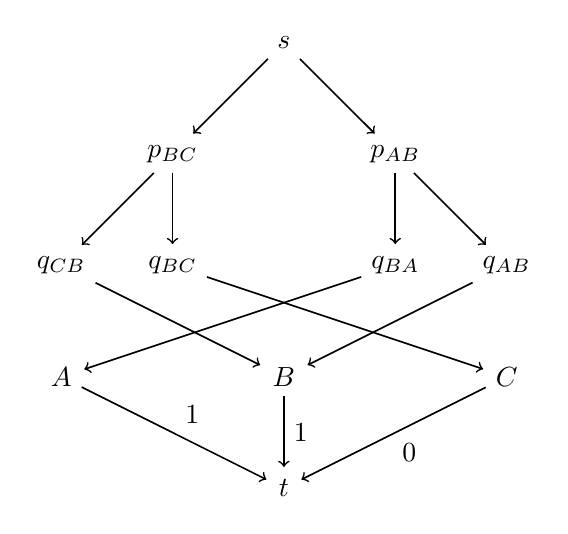
\begin{tikzpicture}[
                    ->,
                    shorten >=1pt,
                    auto,
                    node distance=2.0cm,
                    semithick
                ]
                \node (S)   {$s$};
                \node (AB)  [below right of=S]                         {$p_{AB}$};
                \node (BC)  [below left  of=S]                         {$p_{BC}$};
                \node (ABe) [below right of=AB]                        {$q_{AB}$};
                \node (BAe) [below       of=AB, node distance=1.414cm] {$q_{BA}$};
                \node (BCe) [below       of=BC, node distance=1.414cm] {$q_{BC}$};
                \node (CBe) [below left  of=BC]                        {$q_{CB}$};
                \node (A)   [below       of=CBe,node distance=1.414cm] {$A$};
                \node (B)   [right       of=A,  node distance=2.828cm] {$B$};
                \node (C)   [below       of=ABe,node distance=1.414cm] {$C$};
                \node (T)   [below       of=B,  node distance=1.414cm] {$t$};

                \path
                (S) edge node {} (AB)
                (S) edge node {} (BC)
                (BC) edge node {} (CBe)
                (BC) edge node {} (BCe)
                (AB) edge node {} (BAe)
                (AB) edge node {} (ABe)
                (CBe) edge node {} (B)
                (BCe) edge node {} (C)
                (BAe) edge node {} (A)
                (ABe) edge node {} (B)
                (A) edge node {$1$} (T)
                (B) edge node {$1$} (T)
                (C) edge node {$0$} (T)
                ;
            \end{tikzpicture}

            \label{fig:flownetwork}

            \caption{
                The flow network corresponding to the simple graph in figure
                \ref{fig:graph}. All edges have capacity $1$ unless otherwise
                indicated.
            }
        \end{figure}

    \item The following linear program determines the minimum weight of food
        to pack while satisfying all of Gerlinde Kaltenbrunner's requirements.

        \begin{align*}
            \text{minimize} \quad
                & x_A + x_B + x_C + x_D + x_E                                                         \\
            \text{subject to} \quad
                & T    \leq (5000)(21)                                                                \\
                & 0.50 \leq \frac{2500x_A + 1500x_B + 2500x_C + 3500x_D + 1000x_E}{T} \leq 0.65       \\
                & 0.20 \leq \frac{3500x_A + 100x_B  + 100x_C  + 1800x_D + 2900x_E}{T} \leq 0.35       \\
                & 0.15 \leq \frac{500x_A  + 3500x_B + 2500x_C + 200x_D  + 500x_E }{T} \leq 0.20       \\
                & x_A  \geq 0                                                                         \\
                & x_B  \geq 0                                                                         \\
                & x_C  \geq 0                                                                         \\
                & x_D  \geq 0                                                                         \\
                & x_E  \geq 0                                                                         \\
            \text{where} \quad
                & T    = (2500 + 3500 + 500) x_A + (1500 + 100 + 3500) x_B + (2500 + 100 + 2500) x_C  \\
                &      + (3500 + 1800 + 200) x_D + (1000 + 2900 + 500) x_E
        \end{align*}

    \item

        \begin{enumerate}
            \item Draw the feasible region of the linear program.

                \begin{figure}[H]
                    \centering
                    \includegraphics[width=0.5\textwidth]{plot.pdf}
                \end{figure}

            \item The following list has the a vertex of the feasible region in
                each row of the left column and its defining two equations in
                the right column.

                \begin{align*}
                    (0, 2)  &\quad (3, 5) \\
                    (2, 3)  &\quad (2, 5) \\
                    (3, 1)  &\quad (2, 4) \\
                    (0, 0)  &\quad (1, 4) \\
                    (-1, 1) &\quad (1, 3)
                \end{align*}

            \item To maximize the objective function given by $x_1 + 2x_2$, the
                simplex algorithm would proceed in one of the two following
                ways if it starts at $(x_1, x_2) = (0, 0)$.

                \begin{enumerate}
                    \item
                        \begin{enumerate}
                            \item
                                Set inequality $1$ to equality
                                and move to better feasible point $(-1, 1)$.
                            \item
                                Set equality $1$ back to inequality,
                                set inequality $3$ to equality,
                                and move to better feasible point $(0, 2)$.
                            \item
                                Set equality $3$ back to inequality,
                                set inequality $5$ to equality,
                                and move to better feasible point $(2, 3)$.
                            \item
                                Set equality $5$ back to inequality,
                                set inquality $2$ to equality. \\
                                There are no better feasible points along that
                                line,
                                so set equality $2$ back to inequality. \\
                                $(2, 3)$ is the optimum.
                        \end{enumerate}

                    \item
                        \begin{enumerate}
                            \item
                                Set inequality $4$ to equality
                                and move to better feasible point $(3, 1)$.
                            \item
                                Set equality $4$ back to inequality,
                                set inequality $2$ to equality,
                                and move to better feasible point $(2, 3)$.
                            \item
                                Set equality $2$ back in equality
                                and set inequality $5$ to equality. \\
                                There are no better feasible points along that
                                line,
                                so set equality $5$ back to inequality. \\
                                $(2, 3)$ is the optimum.
                        \end{enumerate}
                \end{enumerate}
        \end{enumerate}

    \item We wish to show a proposition about the line between two feasible
        solutions.

        \begin{proposition}
            If $x,x^\prime \in \R^n$ are feasible solutions to a given linear
            program, then all points on the line between $x$ and $x^\prime$ are
            also solutions to that linear program.
        \end{proposition}

        \begin{proof}
            First suppose all constraints in the linear program are of the form
            $$
            x \cdot a \leq b
            $$
            where $a \in \R^n$ and $b \in \R$.

            Second, all points on the line between $x$ and $x^\prime$ are identified by
            $\alpha \in [0,1]$ as follows.
            $$
            \alpha x + (1-\alpha)x^\prime
            $$

            Third, we examine some resulting inequalities.
            \begin{align}
                (1 - \alpha)x^\prime \cdot a & \leq (1 - \alpha) b \label{ineq:oneminusalphax} \\
                \alpha x \cdot a \leq \alpha b \label{ineq:alphax}
            \end{align}

            Finally, we consider the following equality, which is a
            reformulation of what it means to lie on the line between $x$ and
            $x^\prime$.
            \begin{align}
                (\alpha x \cdot a + (1 - \alpha) x^\prime) \cdot a
                &= \alpha x \cdot a + (1 - \alpha) \cdot a \notag \\
                &= \alpha x \cdot a + x^\prime \cdot a - \alpha x^\prime \cdot a \label{eq:qed}
            \end{align}

            Adding up inequalities \eqref{ineq:oneminusalphax} and
            \eqref{ineq:alphax}, we arrive at the statement we wish to prove,
            which completes the proof.

            Alternatively, suppose that a point on the line between $x$ and
            $x^\prime$ were not a feasible solution. Geometrically, that would
            be a contradiction of the convexity of the feasible region. Hence,
            all points on a line between any two feasible solutions must be
            feasible solutions.
        \end{proof}

    \item For a graph in which each edge is given a load and the load of a
        vertex is given by the sum of the loads of its edges, we seek to find
        an assignment of edges loads that sum to $1$ but minimize the maximal
        vertex load. To do so with linear programming, the set of variables
        consists of the edge loads as well as an additional variable to
        represent the maximal vertex load due to the current assignment of edge
        loads.

        \begin{enumerate}
            \item For a graph on four vertices $a$, $b$, $c$, $d$ with edges
                $(a, b)$, $(a, c)$, $(b, c)$, $(b, d)$, $(c, d)$, solutions
                to the following linear program provide assignments to the
                edge loads that minimize the maximum load on any vertex.

                \begin{align*}
                    \text{minimize} \quad &
                        M \\
                    \text{subject to} \quad
                        & M \geq x_{ab} + x_{ac} \\
                        & M \geq x_{ab} + x_{bc} + x_{bd} \\
                        & M \geq x_{ac} + x_{bc} + x_{cd} \\
                        & M \geq x_{bd} + x_{cd} \\
                        & x_{ab} + x_{ac} + x_{bc} + x_{bd} + x_{cd} = 1 \\
                        & M \geq 0 \\
                        & x_{ab} \geq 0 \\
                        & x_{ac} \geq 0 \\
                        & x_{bc} \geq 0 \\
                        & x_{bd} \geq 0 \\
                        & x_{cd} \geq 0
                \end{align*}

            \item The dual of the above linear program is the following.

                \begin{align*}
                    \text{maximize} \quad
                        & (0, 0, 0, 0, 1, -1) y \\
                    \text{subject to} \quad &
                    \left(
                        \begin{array}{cccccc}
                            1  & 1  & 1  & 1  & 0 & 0 \\
                            -1 & -1 & 0  & 0  & 1 & -1 \\
                            -1 & 0  & -1 & 0  & 1 & -1 \\
                            0  & -1 & -1 & 0  & 1 & -1 \\
                            0  & -1 & 0  & -1 & 1 & -1 \\
                            0  & 0  & -1 & -1 & 1 & -1
                        \end{array}
                    \right)
                    y
                    \leq
                    \left(
                        \begin{array}{c}
                            1 \\
                            0 \\
                            0 \\
                            0 \\
                            0 \\
                            0
                        \end{array}
                    \right)
                \end{align*}

                In order, the rows of the dual matrix are due to $M$, $x_{ab}$,
                $x_{ac}$, $x_{bc}$, $x_{bd}$, $x_{cd}$.

            \item Now, we formulate the problem for a general graph
                $G = (V, E)$.

                The variables of the program in this case are $x_{uv}$
                for each $\{u, v\} \in E$, i.e. the loads given to each edge.
                We define the load on a vertex as
                $$
                l_v = \sum_{\{u, v\}} {l_{\{u, v\}}}
                $$
                i.e. the sum of the loads on the vertex's adjacent edges.

                The linear program is the following.
                \begin{alignat*}{3}
                    \text{minimize} \quad
                        & M \\
                    \text{subject to} \quad
                        & M \geq l_v & \text{for } v \in V \\
                        & \sum_{e \in E} l_e = 1 \\
                        & M \geq 0 \\
                        & l_e \geq 0 & \text{for } e \in E
                \end{alignat*}
        \end{enumerate}

    \item We wish to find solutions to systems of linear equations that are
        maximimally flat, i.e. that minimize the maximal difference $x_i - x_j$
        in the solution vector. The linear program that accomplishes that is
        the following.

        \begin{alignat*}{3}
            \text{minimize} \quad
                & M \\
            \text{subject to} \quad
                & A x = b \\
                & M \geq x_i - x_j \quad
                & \text{for } i = 1, \dots, n
        \end{alignat*}
        where $A$ is the matrix of coefficients of the linear systems and $n$
        is the size of the vectors $x$ and $b$.

\end{enumerate}

\end{document}
